\chapter{Overview of medical imaging}
- standard computer vision methods
- machine learning methods
\section{Computed tomography}
Neuroimaging is crucial when aiming for an exact diagnosis of intracranial hemorrhage.  Taking into account its wide availability and non-invasive technique, computed tomography (CT) is most commonly used in detection of intracranial hemorrhage these days \cite{imagingICH}. Even though magnetic resonance imaging (MRI) has been proved to be more sensitive, CT is able to provide much faster results, which is critical when it comes to obtaining early assessment of the presence and extent of the bleeding \cite{imagingAfterBrainInjury}. The main principle of non-contrast computed tomography imaging resides in the fact, that different tissues of the human body can absorb different amounts of X-ray beams, which is refferd to as tissue density \cite{principlesOfCT}. The absorbed X-ray is being mapped into Hounsfield Units (HU). Resulting scans are formed from units of space within the patient's body called voxels. These units contain a three-dimensional (3D) information about the value of tissue density. Resulting 3D scans are studied using a method called windowing, which converts selected range of Hounsfield Units (HU) into values of grayscale (range between 0 and 255).  As a result, a two-dimensional cross sectional "slice" can be extracted from the 3D volume. The selected range is set by two different parameters: window width (WW) and window level (WL). Windowing enables radiologists to study different features and tissues by increasing the contrast, thus bringing forward the tissue of interest \cite{windowClassBiomArt}. The original CT pixel values, which are not in the selected range, are displayed either as black or white, as shown in Figure 2.2 .

\begin{figure}[h]
\begin{centering}
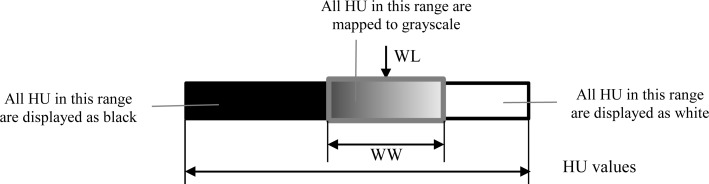
\includegraphics[width=15cm]{assets/images/windowingHU}
\par\end{centering}
\caption{Windowing of CT scans \cite{windowClassBiomArt}
\label{fig:windowing}}
\end{figure}

In detection of intracranial hemorrhage from head CT scans, blood and brain windows are the standard choice. Right after the appearance of hemorrhage, the area of the bleeding shows density values of 60 to 80 Hounsfield units (HU), and as it matures, the value increases up to 100 HU  \cite{principlesOfCT}, which can be visible with a correct setting of window width and window length.
\chapter{Deep learning}
\section{Convolutional neural networks}

% \say{Here, a quotation is written and even some \say{nested} quotations 
% are possible}

% Figure \ref{fig:dynabook}:

% \begin{figure}[h]
% \begin{centering}
% 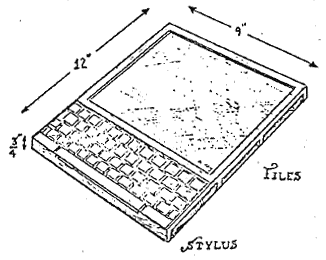
\includegraphics[width=5cm]{assets/images/Dynabook}
% \par\end{centering}
% \caption{Dynabook \label{fig:dynabook}}
% \end{figure}